\chapter{Установка ОС на целевую платформу}
\textbf{Цель:} Установить дистрибутив Debian 10 на целевую платформу.

\textbf{Описание:} Нужно понимать, что ОС Linux делиться на две части. Ядро (Kernel) и файловую систему (rootfs). Ядро определяет какие возможности по взаимодействию с железом доступны пользователю и приложениям. Rootfs определяет какие инструменты есть в системе, порядок инициализации, запуска сервисов и прочие прикладные штуки. Дистрибутив это в большей степени наполнение rootfs. Не каждый дистрибутив имеет поддержку иной от x86 архитектур.

Для установки debian воспользуемся инструментом под названием debootstrap, который отвечает за создание rootfs. Подробнее про этот инструмент, и возможности по его управлению, Вы можете найти на wiki проекта Debian.


\section{Подготовка rootfs}

\subsection{}Запустите виртуальную машину. Логин и пароль для входа: student / usrstudent.

\subsection{} Запустите консоль нажав комбинацию клавиш на клавиатуре \textbf{Ctrl+Alt+T} \\

\textbf{Внимание!} В консоли есть возможность автоматического продолжения ввода. Для этого необходимо ввести первые символы команды, или пути, и нажать клавишу TAB. Ввод продолжиться до тех пор, пока не появиться неопределённостью (к примеру у Вас есть два файла foo\_bar1 и foo\_bar2, при нажатии TAB будет вставлен текст до цифры). Двойное нажатие TAB приведёт к выводу всех возможных вариантов продолжения, если таковые есть.

\subsection{}Создайте и перейдти в рабочий каталог в котором будет создан образ rootfs.
\begin{lstlisting}[style=bash]
# mkdir -p $BAGET/lab_01
# cd $BAGET/lab_01 
\end{lstlisting}

\subsection{} Запустите утилиту debootstrap (при необходимсоти введите пароль usrstudent):
\begin{lstlisting}[style=bash]
# sudo debootstrap --include=aptitude,nano,wget \
--foreign \
--arch=mips64el buster rootfs
\end{lstlisting}
\textit{-{}-include=A,B,C..} - добавить в сборку указанные пакеты \\
\textit{-{}-foreign} — только сгенерировать наполнение, применяется когда архитектура на которой запускается утилита отлична от архитектуры назначения. \\
\textit{-{}-arch=mips64el} — указываем целевую архитектуру \\
\textit{buster} — версия сборки \\
\textit{rootfs} — путь к папке назначения, где будут размещены файлы \\

\subsection{} Для продолжения установки, нам понадобиться утилита qemu позволяющая эмулировать различные архитектуры. Скопируем исполняемый файл qemu:
\begin{lstlisting}[style=bash]
# sudo cp /usr/bin/qemu-mips64el-static ./rootfs/usr/bin
\end{lstlisting}
и перейдём в созданную rootfs (привет дедушка контейнеров, chroot)
\begin{lstlisting}[style=bash]
# sudo chroot ./rootfs
\end{lstlisting}



\section{Настройка rootfs}

\subsection{} Завершим работу debootstrap
\begin{lstlisting}[style=bash]
# export LANG=en_US.UTF-8
# /debootstrap/debootstrap --second-stage
\end{lstlisting}

\subsection{}Добавим источники для установки ПО, для этого выполним следующие команды 
\begin{lstlisting}[style=bash]
# echo deb http://ftp.debian.org/debian buster \
main contrib non-free  >> /etc/apt/sources.list

# echo deb-src http://ftp.debian.org/debian buster \
main contrib non-free >> /etc/apt/sources.list

# echo deb http://ftp.debian.org/debian buster-updates \
main contrib non-free >> /etc/apt/sources.list

# echo deb-src http://ftp.debian.org/debian buster-updates \
main contrib non-free >> /etc/apt/sources.list
\end{lstlisting}

\subsection{} Обновим список, и установим ряд приложений
\begin{lstlisting}[style=bash]
# apt-get update
# apt-get install -y dialog sudo less i2c-tools evtest mc \
openssh-server resolvconf hwinfo net-tools
\end{lstlisting}

\subsection{}Зададим пароль для root пользователя
\begin{lstlisting}[style=bash]
# passwd root
\end{lstlisting}
После чего введите root (внимание, курсор двигаться не будет, это политика безопасности Linux, при вводе пароля курсор не перемещается, что бы нельзя было установить количество символов). И нажмите Enter

Затем Вас попросят повторить пароль, снова введите root и нажмите Enter

\subsection{}Настроим работу сетевого интерфейса со статическим адресом, для этого создадим файл в паке /etc/network/interfaces.d/

\begin{lstlisting}[style=bash]
# nano /etc/network/interfaces.d/eth0
\end{lstlisting}
и впишите туда следующие строки:

\begin{lstlisting}[style=stdout]
auto eth0
	iface eth0 inet static
	address 192.168.100.200
	netmask 255.255.255.0
	network 192.168.100.0
\end{lstlisting}

Первая строка определяет когда настраивается интерфейс. Auto означает, что при загрузке ОС. 
Для USB адаптеров, лучше выбирать allow-hotplug, что бы сократить время загрузки ОС. 

Вторая строка определяет, что мы будем использовать статический ip адрес, 
далее идёт конфигурация адресов.

Выходим из редактора nano, нажав комбинацию клавиш Ctrl+X. Вам будет задан вопрос о сохранении изменения в файле, жмём Y и клавишу Enter.

\subsection{}Настроим имя компьютера

\begin{lstlisting}[style=bash]
# echo baget > /etc/hostname
\end{lstlisting}

\subsection{}Завершим настройку rootfs

\begin{lstlisting}[style=bash]
# exit
# sudo rm ./rootfs/usr/bin/qemu-mips64el-static
\end{lstlisting}

\subsection{}Скопируйте папку barebox из каталога support в корень созданной rootfs
\begin{lstlisting}[style=bash]
# sudo cp -r $BAGET/support/barebox/ ./rootfs/
\end{lstlisting}

В данной папке лежит скомпилированное ядро Linux (vmlinux…), скомпилированное дерево устройств (k5500vk018\_rbm.dtb) и скрипт выполняемый загрузчиком (barebox.sh).



\section{Проверка}

\subsection{}Вставьте SD карту в ПК, и подключите её к виртуальной машине
\begin{center}
	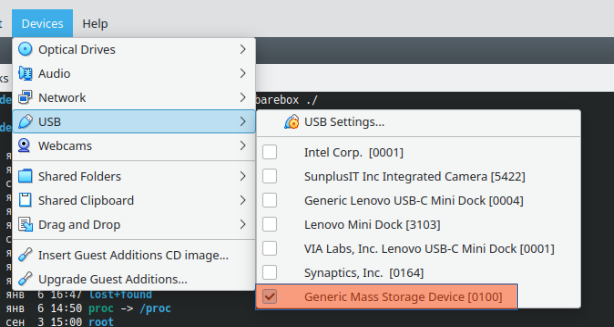
\includegraphics[width=\textwidth]{pic_04}
\end{center}

\subsection{}Необходимо узнать точку монтирования SD карты. Она может отличаться в зависимости от ридера, что Вы используете. Для упрощения ввода, выполните команду в консоле:
\begin{lstlisting}[style=bash]
# mount | grep ^/dev
\end{lstlisting}
для получения списка примонтированных устройств, при этом командой grep происходит фильтрация лишнего вывода, и отображается только список блочных устройств. Вывод будет примерно как на рисунке

\begin{center}
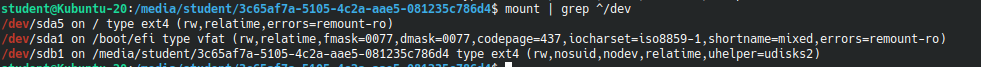
\includegraphics[width=\textwidth]{pic_05}
\end{center}

Первые две строчки, это разделы виртуального жёсткого диска, далее точка монтирования SD карты (/media/student/…)

Для упрощения ввода, создадим временную системную переменную, которой назначим путь, для примера\textbf{(!)} на рисунке выше:
\begin{lstlisting}[style=bash]
# export BAGET_SD=\
/media/student/3c65af7a-5105-4c2a-aae5-081235c786d4
\end{lstlisting}

Нужно помнить, что эта переменная существует только в том терминале, где был вызван export, в остальных окнах терминала она не существует, если Вы закроете текущее окно, или Вам понадобиться эта переменная в другом окне, необходимо будет повторить процедуру присвоения.

\subsection{}Удалите все файлы с sd карты
\begin{lstlisting}[style=bash]
# sudo rm -rf $BAGET_SD/*
\end{lstlisting}
скопируйте созданную rootfs на sd карту
\begin{lstlisting}[style=bash]
# sudo cp -a $BAGET/lab_01/rootfs/* $BAGET_SD/
\end{lstlisting}
и отмантируйте SD карту 
\begin{lstlisting}[style=bash]
# sudo umount $BAGET_SD
\end{lstlisting}
(это важно, так как в ОС Linux запись данных на носители происходит в фоне, и если вы отключите накопитель «неправильно» то нет гарантии, что данные успели записаться на носитель!).
Дождитесь когда команда выполниться, после чего достаньте SD карту и вставьте её в плату.

\subsection{}Подключите USB шнуром плату к ПК. Проверьте, и при необходимости подключите USB устройство FTDI RBM\_C1K5500VK018 к виртуальной машине (меню Device→USB).

\subsection{} Запустите программу gtkterm или нажмите Ctrl + Shift + T для открытия новой вкладки в окне терминала и выполните команду minicom (это консольная утилита, в виртуальной машине эта утилита уже настроена на нужный порт, с нужными параметрами)
\begin{center}
	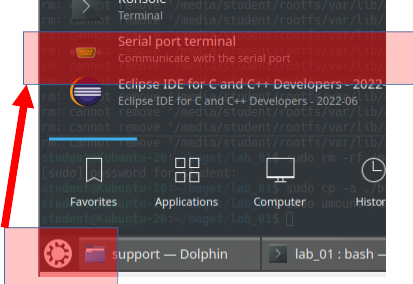
\includegraphics[width=\textwidth]{pic_06}
\end{center}

\subsection{} Выберите порт  /dev/ttyUSB1 через меню Configuration->Port.
\begin{center}
	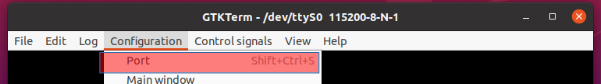
\includegraphics[width=\textwidth]{pic_07}
\end{center}

Нажмите кнопку OK.

сли в окне не появился текст, и на нажатие клавиши Enter так же нет реакции,  нажмите на кнопку Reset на плате. Изучите вывод, там будет написано, что пошло не так.

Один из вариантов, когда при записи файлов на SD карту что-то побилось. В этом случае, вы увидите много записей как в примере ниже:
\begin{lstlisting}[style=stdout]
srisa-sdhci 1b50b000.sdhci@1b50b000.of: registered as mci0
srisa-sdhci 1b50b000.sdhci@1b50b000.of: SDHCI timeout while waiting for done
srisa-sdhci 1b50b000.sdhci@1b50b000.of: error on command 8
srisa-sdhci 1b50b000.sdhci@1b50b000.of: state = 0400 03ff, interrupt = 8001 0001
srisa-sdhci 1b50b000.sdhci@1b50b000.of: r0 00000000 r1 00000000 r2 00000000 r3 00000000
\end{lstlisting}

Нужно повторить все шаги этого раздела. \textbf{При вынимании SD карты убедитесь, что плата обесточена!}

\subsection{} Введите в качестве логина и пароля root

Поздравляем, Вы запустили Debian дистрибутив на плате.

\subsection{} Выключите плату, для чего в начале введите команду
\begin{lstlisting}[style=bash]
$ poweroff
\end{lstlisting}
дождитесь, как появиться надпись
\begin{lstlisting}[style=stdout]
reboot: System halt
\end{lstlisting}
после чего отключите USB кабель от ПК или платы. 